% =====================================================================
%  CSE499A — EHR Pre-Consultation Medical Documentation System
%  Standalone section: Project Design
%  (System Design + Tools/Components + Implementation)
%  Authors: Rafiur Rahman Mashrafi (2221971042),
%           M.G. Rabbi Hossen (2222516042),
%           Israt Zaman Srity (2211084042)
%  Advisor: Dr. Mohammad Ashrafuzzaman Khan [AzK]
%  Department of Electrical and Computer Engineering,
%  North South University · Spring 2026
% =====================================================================

\documentclass[12pt,a4paper]{article}

\usepackage[utf8]{inputenc}
\usepackage[T1]{fontenc}
\usepackage{mathptmx}
\usepackage[a4paper,margin=1in]{geometry}
\usepackage{setspace}
\usepackage{enumitem}
\usepackage{booktabs}
\usepackage{longtable}
\usepackage{tabularx}
\usepackage{ragged2e}
\usepackage{array}
\usepackage{tikz}
\usepackage[hidelinks]{hyperref}
\usepackage{titlesec}
\usepackage{xcolor}
\usepackage{caption}

\usetikzlibrary{shapes,shapes.geometric,arrows,arrows.meta,positioning}

\onehalfspacing
\setlength{\parskip}{6pt}
\setlength{\parindent}{1.5em}

\titleformat{\section}{\normalfont\large\bfseries}{\thesection}{0.7em}{}
\titleformat{\subsection}{\normalfont\normalsize\bfseries}{\thesubsection}{0.7em}{}

\title{\bfseries Project Design:\\
EHR-Based Pre-Consultation Medical Documentation System}
\author{Rafiur Rahman Mashrafi (ID 2221971042)\\
        M.~G.~Rabbi Hossen (ID 2222516042)\\
        Israt Zaman Srity (ID 2211084042)\\[6pt]
        \emph{Faculty Advisor:} Dr. Mohammad Ashrafuzzaman Khan [AzK]\\
        Department of Electrical and Computer Engineering\\
        North South University, Bangladesh}
\date{Senior Design Project (CSE499A) \quad Spring 2026}

\begin{document}
\maketitle

\section{Introduction}

This section presents the project design of the
\textit{EHR-Based Pre-Consultation Medical Documentation System}.
The design is described in three layers: (i)~the system architecture
--- the end-to-end pipeline that turns Bangla speech into a
structured Electronic Health Record (EHR); (ii)~the hardware and
software components used to realise the pipeline; and (iii)~the
implementation methodology, organised around the five operational
phases of CSE499A. The aim is to provide a complete, reproducible
description of what the system is, what it is built from, and how
it has been built so far.

\section{System Design}

\subsection{Overall pipeline}
The system is a five-stage pipeline that converts a patient's spoken
description into a structured EHR record presented to the attending
physician. Figure~\ref{fig:pipeline} shows the overall block
diagram. The patient interacts only with Stage~1; Stages~2--4 run on
a backend service; the physician interacts only with Stage~5. The
original audio transcript is preserved alongside the structured
record and is always visible on the doctor's dashboard so that any
extracted entity can be traced back to the speech that produced it.

\begin{figure}[h!]
\centering
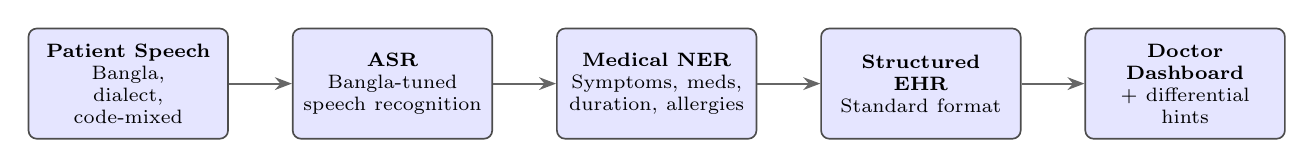
\begin{tikzpicture}[
  node distance=10mm and 8mm,
  stage/.style={rectangle, rounded corners=3pt, draw=black!70,
                fill=blue!10, line width=0.6pt,
                text width=23mm, minimum height=14mm,
                align=center, font=\scriptsize\bfseries},
  arrow/.style={-Stealth, line width=0.7pt, black!60}
]
\node[stage] (s1) {Patient Speech\\\scriptsize\mdseries Bangla,\\dialect, code-mixed};
\node[stage, right=of s1] (s2) {ASR\\\scriptsize\mdseries Bangla-tuned\\speech recognition};
\node[stage, right=of s2] (s3) {Medical NER\\\scriptsize\mdseries Symptoms, meds,\\duration, allergies};
\node[stage, right=of s3] (s4) {Structured\\EHR\\\scriptsize\mdseries Standard format};
\node[stage, right=of s4] (s5) {Doctor\\Dashboard\\\scriptsize\mdseries +~differential\\hints};

\draw[arrow] (s1) -- (s2);
\draw[arrow] (s2) -- (s3);
\draw[arrow] (s3) -- (s4);
\draw[arrow] (s4) -- (s5);
\end{tikzpicture}
\caption{Block diagram of the proposed pre-consultation EHR pipeline.}
\label{fig:pipeline}
\end{figure}

\subsection{Stage 1 --- Patient Speech Capture}
The patient sits at a voice-enabled device (a consumer tablet or a
fixed kiosk) in the clinic waiting area. After a recorded
informed-consent prompt in Bangla, the patient describes their
symptoms, medical history, current medications, and allergies in
natural speech. No structured questionnaire is imposed; the patient
speaks freely. The capture front-end records 16~kHz mono audio,
applies basic gain normalisation, and uploads the audio chunk to the
backend over an authenticated channel. No on-device ASR runs at this
stage.

\subsection{Stage 2 --- Automatic Speech Recognition (ASR)}
The recorded audio is passed to a Bangla-tuned ASR model that
produces a Unicode Bangla transcript. Embedded English words are
preserved as-is rather than normalised away, because Bangla--English
code-mixing is a defining feature of real Bangladeshi clinical
speech and forcing a monolingual transcript would discard
clinically relevant information (medication names, symptom
descriptors, condition names). Long recordings are first
voice-activity-segmented into 10--15~second clips before being fed
to the model, since most evaluated ASR architectures cannot accept
arbitrarily long input. The choice of ASR model is the central
deliverable of CSE499A and is described in detail in
Section~\ref{sec:phases}.

\subsection{Stage 3 --- Medical Named Entity Recognition (NER)}
A medical NER module reads the transcript and labels clinically
relevant spans. The target entity classes are:
\textit{symptom}, \textit{disease}, \textit{medication},
\textit{dosage}, \textit{duration}, \textit{frequency},
\textit{allergy}, and \textit{anatomical site}. The planned
implementation will adapt BanglaBERT with a token-classification
head, trained on a small annotated corpus to be collected during
CSE499B. NER is not part of the empirical results in CSE499A; the
present report establishes the upstream ASR baseline on which the
NER will operate.

\subsection{Stage 4 --- Structured EHR Construction}
The labelled spans are normalised --- dosage strings to standard
units, durations to ISO~8601-like intervals --- and packaged into a
structured record. The schema includes a patient identifier, a
recording timestamp, the chief complaint, a list of symptoms with
onset and duration, a medication list, an allergy list, and a free
text \texttt{notes} field that contains the verbatim transcript so
that nothing is hidden from the physician. The schema design will
be informed by Phase~5 of the project, in which several public AI
chatbots are prompted with simulated patient utterances and their
EHR-style outputs are compared.

\subsection{Stage 5 --- Doctor Dashboard with Differential Hints}
The physician sees a clean web interface that displays the
structured record, the original transcript, and a short list of
differential-diagnosis hints derived from a lightweight medical
knowledge layer. For example, a transcript reporting persistent
cough together with night sweats and weight loss would surface
``possible tuberculosis, consider ruling out lung pathology'' as a
hint. The system never renders a diagnosis: it only narrows the
search space. The physician can confirm, override, or annotate the
record, and all changes are versioned. Final clinical authority and
legal responsibility remain with the licensed physician.

\subsection{Design properties}
Three properties were enforced throughout the architecture.
\textit{Auditability}: every extracted entity is traceable back to
the audio segment it came from, so there are no silent edits or
untraceable model ``corrections.''
\textit{Honest accuracy reporting}: model accuracy is reported on
real dialect speech rather than on clean read-aloud benchmarks, so
the physician sees an honest estimate of system reliability.
\textit{Decision-support boundary}: the system assists the
physician but does not replace the physician's clinical judgement.

\section{Hardware and Software Components}

This is a software-only project; no custom hardware has been
fabricated. The patient-facing capture device, in deployment, would
be a consumer Android tablet (typical 8--10$^{\prime\prime}$ form
factor) or a fixed kiosk built around the same hardware. All model
evaluation and development was performed on free-tier Google Colab
GPU instances. Table~\ref{tab:tools} lists the principal software
components and the rationale for each selection.

\renewcommand{\arraystretch}{1.2}
\footnotesize
\begin{longtable}{>{\raggedright\arraybackslash}p{2.6cm}
                  >{\raggedright\arraybackslash}p{3.3cm}
                  >{\raggedright\arraybackslash}p{2.7cm}
                  >{\raggedright\arraybackslash}p{4.6cm}}
\caption{Software tools and components used.}\label{tab:tools}\\
\toprule
\textbf{Tool} & \textbf{Function} & \textbf{Similar tools} & \textbf{Why this one} \\
\midrule
\endfirsthead
\multicolumn{4}{c}{\itshape Table~\ref{tab:tools} continued}\\
\toprule
\textbf{Tool} & \textbf{Function} & \textbf{Similar tools} & \textbf{Why this one} \\
\midrule
\endhead
\midrule
\multicolumn{4}{r}{\itshape continued on next page}\\
\endfoot
\bottomrule
\endlastfoot
Python 3.10 & Implementation language & R, Julia & Standard for ML/NLP; widest ecosystem of speech and NLP libraries. \\
PyTorch 2.x & Deep-learning framework & TensorFlow, JAX & Native support across all evaluated ASR models; preferred by Hugging Face. \\
HF Transformers~\cite{pd:transformers} & Model loading, inference, tokenisation & ESPnet, NeMo & Single unified API across Whisper, Wav2Vec2, MMS, SeamlessM4T, Qwen-Audio, Voxtral, Phi-4. \\
HF Datasets, Accelerate, PEFT & Streaming, mixed-precision inference, planned LoRA fine-tuning & Custom data pipelines, DeepSpeed & Lowest friction with Transformers; PEFT~\cite{pd:lora} is the planned fine-tuning route. \\
Librosa, SoundFile, FFmpeg & Audio I/O, 16~kHz resampling, mono conversion & torchaudio, sox & Stable, well-documented; run reliably on Colab. \\
WhisperX~\cite{pd:whisperx} & Long-form audio segmentation and forced alignment & pyannote.audio & Required for transcribing audio longer than Whisper's 30-second window. \\
\texttt{jiwer}, \texttt{evaluate} & Computing WER, CER, BLEU & sclite (NIST) & Pure-Python; standard for speech evaluation. \\
yt-dlp & Public-source audio collection & youtube-dl & Maintained fork; reliable for dialect audio sourcing. \\
Google Colab (T4, A100) & Primary GPU compute & Kaggle, local GPU & Free tier sufficient for inference benchmarks. \\
Google Drive & Dataset and checkpoint storage & S3, local NAS & Free integration with Colab; sufficient for $\sim$5~GB project data. \\
Git / GitHub & Source control and project repository & GitLab, Bitbucket & Standard; required for reproducibility and submission. \\
\end{longtable}
\normalsize

\subsection{Planned components for the deployed system}
The CSE499B implementation will add a thin application layer above
the model pipeline:

\begin{itemize}[leftmargin=*]
\item \textbf{FastAPI backend (Python)} --- REST/WebSocket service
that receives audio chunks, runs the ASR and NER models, persists
the EHR, and serves it to the dashboard.
\item \textbf{PostgreSQL with at-rest encryption} --- the EHR store;
audio blobs are kept on encrypted object storage.
\item \textbf{React / Next.js dashboard} --- the doctor-facing
interface, designed for low-bandwidth tablets.
\item \textbf{Flutter or PWA patient app} --- the kiosk front-end,
designed for low-tech-literacy users with a single record button
and a Bangla voice prompt.
\item \textbf{JWT authentication and role-based access control} ---
distinct roles for patients (no read access), nurses (intake only),
physicians (full record), and administrators (no clinical content).
\end{itemize}

These components are listed for completeness; their detailed design
falls within CSE499B and is not part of the present report.

\section{Implementation Methodology}
\label{sec:phases}

The CSE499A work was organised around five operational phases, each
closed by a demonstration to the faculty advisor. The phases below
correspond directly to the milestones on the project Gantt chart and
to the deliverables in the project repository.

\subsection*{Phase 1 --- Audio collection and preprocessing}
\textit{Demo 1: 12 March 2026.}
A multi-dialect Bangla audio corpus was assembled from publicly
available recordings covering five regional varieties: Puran Dhaka
(Dhakaiya), Barishali, Sylheti, Normal Bangla, and Indian Bangla.
Each file was renamed under a fixed convention of the form
\texttt{[dialect]\_[index]\_[gender]\_[age].mp3} and logged in
\texttt{dataset\_log.csv} with source, dialect code, speaker gender,
approximate age, and duration. The corpus was then preprocessed:
resampled to 16~kHz mono PCM, RMS-normalised, and segmented into
10--15-second clips by WhisperX's voice-activity detector. The final
corpus is approximately 4.7 hours, 10 source files, $\sim$1{,}100
evaluation segments.

\subsection*{Phase 2 --- Baseline ASR benchmark (12 models)}
\textit{Demo 2: 2 April 2026.}
Twelve open-source Bangla and multilingual ASR models were
benchmarked on the corpus: Whisper Small/Medium/Large/Turbo,
Wav2Vec2 (XLSR-53, 300M, Common-Voice-Bengali variants), MMS,
Vakyansh-Bn, BengaliAI Whisper, BengaliAI Regional, and
SeamlessM4T. Each model transcribed the entire corpus, and
hypothesis transcripts were scored against reference transcripts
using three standard metrics: Word Error Rate (WER), Character
Error Rate (CER), and corpus-level BLEU. Results were recorded in
the project's CSV log. The strongest baseline was BengaliAI
Regional at 46.94\% WER, 24.29\% CER, and 0.273 BLEU. The principal
empirical observation was that even the strongest open Bangla model
gets nearly half the words wrong on dialect speech.

\subsection*{Phase 3 --- Larger multimodal audio LLM benchmark}
\textit{Demo 3: 9 April 2026.}
Following the advisor's instruction to test whether scaling improves
dialect-aware Bangla ASR, six larger 1.7B--7B-parameter multimodal
audio language models were evaluated on the same corpus and same
metrics: Qwen2-Audio (English-routing and direct Bangla modes),
Qwen3-ASR-1.7B, Voxtral-Mini, Phi-4 Multimodal, and Qwen2.5-Omni.
The headline finding was that none of the larger models matched the
smaller specialised baseline; the closest large model trailed
BengaliAI Regional by more than 50 percentage points of WER, and
Phi-4 Multimodal and Qwen2.5-Omni failed to produce usable Bangla
output at all. The conclusion --- ``bigger is not better for Bangla
dialect speech'' --- shaped the methodology for the next phase.

\subsection*{Phase 4 --- Qwen3-ASR fine-tuning research (in progress)}
\textit{Demo 4: 16 April 2026.}
Following the Phase~3 result, the team is currently researching the
methodology for parameter-efficient fine-tuning of
\textbf{Qwen3-ASR-1.7B} on the multi-dialect corpus. The plan,
scheduled for execution in CSE499B, will use LoRA adapters on the
speech encoder while keeping the language-model decoder weights
frozen. No training has been performed yet --- this phase is a
methodology study, not a training run, and the present report is
explicit about that fact.

\subsection*{Phase 5 --- Comparative chatbot output study (selected)}
\textit{Selected: 23 April 2026; execution scheduled for the next demo.}
As a parallel deliverable, several public AI chatbots --- ChatGPT,
DeepSeek, Qwen, Perplexity --- will be prompted with simulated
patient utterances. The structured EHR-style outputs each chatbot
returns will be compared along axes that include schema
consistency, completeness of extracted fields, handling of
code-mixed terms, and faithfulness to the source utterance. The
result will inform the schema design for Stage~4 of the pipeline.
This phase has been selected but is not yet executed and is
therefore not part of the empirical results of CSE499A.

\section{Conclusion}

The project design described above has three layers that work
together: a five-stage architecture that maps spoken Bangla onto a
structured EHR with explicit human-in-the-loop checkpoints; a
software stack chosen for openness, reproducibility, and a near-zero
budget; and a phased implementation methodology that closes the
hardest sub-problem (dialect-aware Bangla ASR) first, then adds the
NER, schema, and dashboard layers in CSE499B. The empirical
benchmarks of Phases~2 and~3 inform the design directly:
specialisation, not scale, is the path forward, and the team has
chosen Qwen3-ASR-1.7B as the target model on which CSE499B's
fine-tuning effort will concentrate.

% =====================================================================
% REFERENCES
% =====================================================================
\begin{thebibliography}{99}

\bibitem{pd:whisper}
A.~Radford \emph{et al.},
``Robust Speech Recognition via Large-Scale Weak Supervision,''
in \emph{Proc.\ ICML 2023}, pp.~28492--28518.
\url{https://arxiv.org/abs/2212.04356}.

\bibitem{pd:mms}
V.~Pratap \emph{et al.},
``Scaling Speech Technology to 1{,}000+ Languages,''
\emph{arXiv:2305.13516}, 2023.
\url{https://arxiv.org/abs/2305.13516}.

\bibitem{pd:wav2vec2}
A.~Baevski \emph{et al.},
``wav2vec 2.0: A Framework for Self-Supervised Learning of Speech
Representations,''
\emph{NeurIPS}, vol.~33, 2020, pp.~12449--12460.
\url{https://arxiv.org/abs/2006.11477}.

\bibitem{pd:qwen2audio}
Y.~Chu \emph{et al.},
``Qwen2-Audio Technical Report,''
\emph{arXiv:2407.10759}, 2024.
\url{https://arxiv.org/abs/2407.10759}.

\bibitem{pd:transformers}
T.~Wolf \emph{et al.},
``Transformers: State-of-the-Art Natural Language Processing,''
in \emph{Proc.\ EMNLP 2020: System Demonstrations}, pp.~38--45.
\url{https://github.com/huggingface/transformers}.

\bibitem{pd:lora}
E.~J.~Hu \emph{et al.},
``LoRA: Low-Rank Adaptation of Large Language Models,''
in \emph{ICLR 2022}.
\url{https://arxiv.org/abs/2106.09685}.

\bibitem{pd:whisperx}
M.~Bain \emph{et al.},
``WhisperX: Time-Accurate Speech Transcription of Long-Form Audio,''
in \emph{INTERSPEECH 2023}.
\url{https://arxiv.org/abs/2303.00747}.

\bibitem{pd:banglabert}
A.~Bhattacharjee \emph{et al.},
``BanglaBERT: Language Model Pretraining and Benchmarks for
Low-Resource Language Understanding Evaluation in Bangla,''
\emph{Findings of NAACL 2022}, pp.~1318--1327.
\url{https://github.com/csebuetnlp/banglabert}.

\bibitem{pd:oodspeech}
F.~R.~Rakib \emph{et al.},
``OOD-Speech: A Large Bengali Speech Recognition Dataset for
Out-of-Distribution Benchmarking,''
\emph{INTERSPEECH 2023}.
\url{https://arxiv.org/abs/2305.09688}.

\end{thebibliography}

\end{document}
